\chapter{実験}
本章では予備実験2種類を含む全9種類の実験について説明を行う.
予備実験として,DCADとレスキュー犬訓練データセットをクリップセットとしてまとめたもののクラス分類を行なった.
犬の一人称動画は人間の一人称動画とは大きく異なる.そのため,この予備実験では犬一人称動画分類タスクに対するCNNの有効性を確認した.

本実験では,sound based three-stream networkを用いてレスキュー犬訓練データセットのマルチクラス推定を行なった.
提案手法の有用性を示すためのアブレーションスタディに
静止画像からのマルチラベル推定,
optical flow画像からのマルチラベル推定,
音声データからのマルチラベル推定2種,
Sound based two-stream networkを用いた音声データと静止画像からのマルチクラス推定,
同じくsound based two-stream networkを用いた音声データとoptical flow画像からのマルチクラス推定
をそれぞれ行なった.
\section{DCAD}
DCADはクリップ毎にフレーム間の平均をとり,画像として扱ってVGG16のpretrained modelを用いてfinetuningを行なった.
予備実験の結果を図~\ref{vgg16_res}に示す.分類率は64.3\%であった.
Iwashitaらによる局所的特徴量を用いた分類実験での精度は60.5\%であった.このことから,犬一人称視点動画においてCNNの有効性が示された.

全般的に,データの多いクラスは精度が高い傾向にあるが,データの少ないクラスは精度が低い傾向にある.
加えて,~\(Car\)クラスは道路の進行方向に対して垂直に待機している10クラスの中で特殊なクラスであり,車などの写ったフレームの影響で分類精度が上昇していると考えられる.~\(Feed\)クラス,~\(Pet\)クラス,~\(Play\_with\_ball\)クラスは,それぞれフレーム内を人間が占める割合が多いクラスと言え,そのため混同が起こりやすいと考えられる.

\begin{figure}[H]
 % \begin{tabular}{cc}
 %  \begin{minipage}{0.5\textwidth}
   \begin{center}

    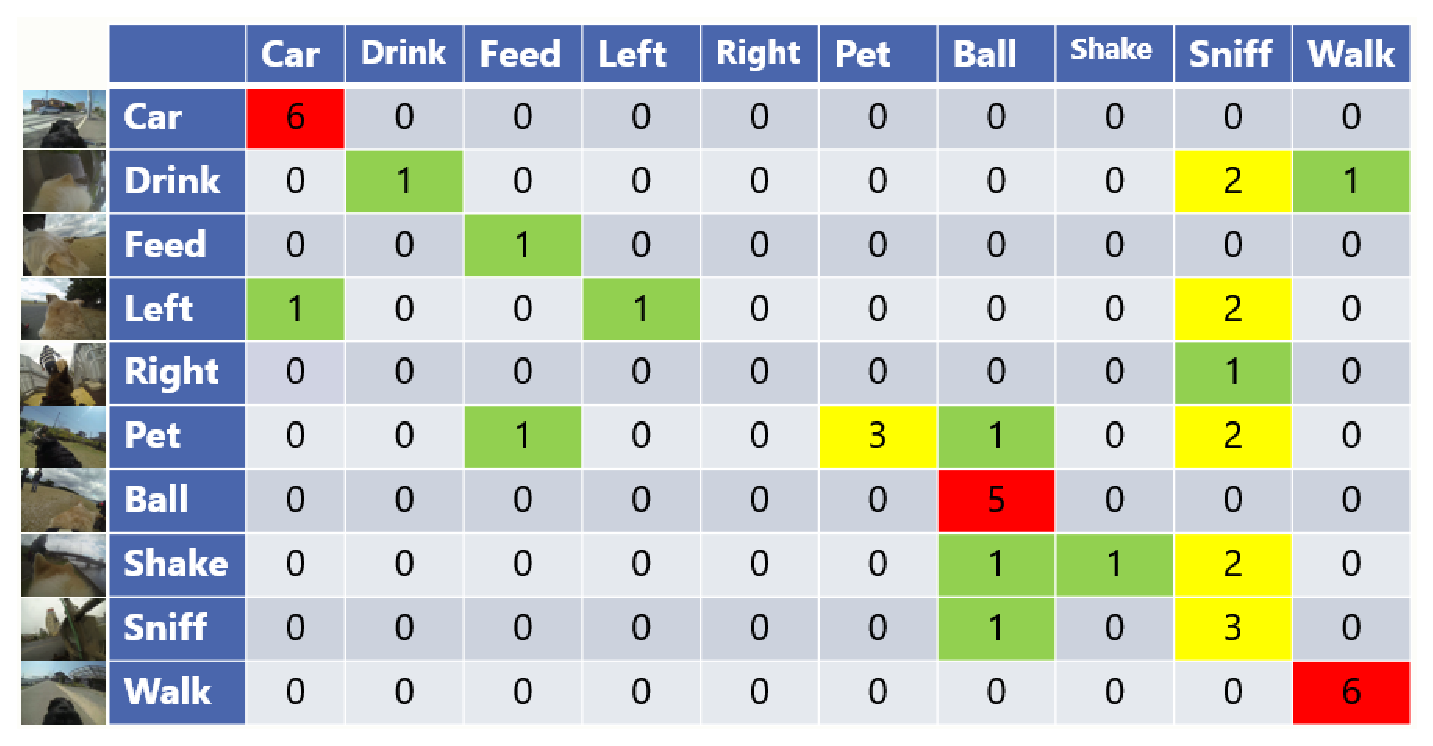
\includegraphics[scale=0.5]{./Figures/vgg16_res.eps}
    \caption{VGG16 pretrained modelとDCADによるfinetuningの結果}
    \label{vgg16_res}
   \end{center}
  % \end{minipage}
  % \begin{minipage}{0.5\textwidth}
\end{figure}

\section{レスキュー犬訓練シングルクラス分類}
レスキュー犬訓練データセットは動画をラベル毎に切り出して短いクリップ群を作り,そのクリップ毎に同様にフレーム間の平均を取った画像を作成しVGG16のpretrained modelを用いてfinetuningした.
\subsection{動画平均画像}
レスキュー犬訓練データセットでの予備実験の結果を図~\ref{sub_resque_res}に示す.

データ数の多いwalkクラスやstopクラスだけでなく,shakeクラスやeatクラスなどのデータ数の少ないクラスも大まかに分類できていることが分かる.
この結果によって,レスキュー犬訓練データセットからクラス分類・推定が可能であることが示された.
\begin{figure}[H]
  \begin{center}
    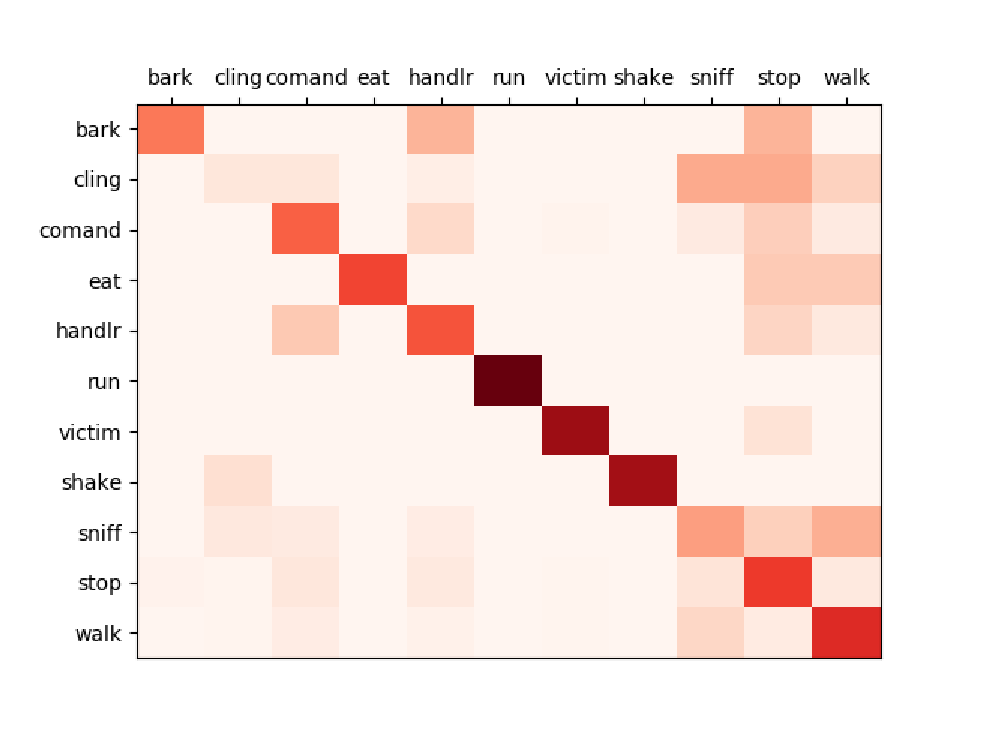
\includegraphics[scale=0.7]{./Figures/resque_mean_result.eps}
    \caption{VGG16 pretrained modelとレスキュー犬訓練データセットフレーム平均画像によるクラス分類のfinetuning結果}
    \label{sub_resque_res}
  \end{center}
\end{figure}

\subsection{オプティカルフロー動画平均画像}
動画像のフレーム間の平均を取った手法と同様に,クリップ毎にoptical flowの平均画像を作成しVGG16のpretrained modelを用いてfinetuningを行なった.
結果を図~\ref{sub_optresque_res}に示す.

やはりデータ数の影響を受けているものの,通常の動画のフレーム平均画像とは異なる傾向が得られた.
この結果によって,optical flow画像から得られる特徴の有用性が示された.
\begin{figure}[H]
  \begin{center}
    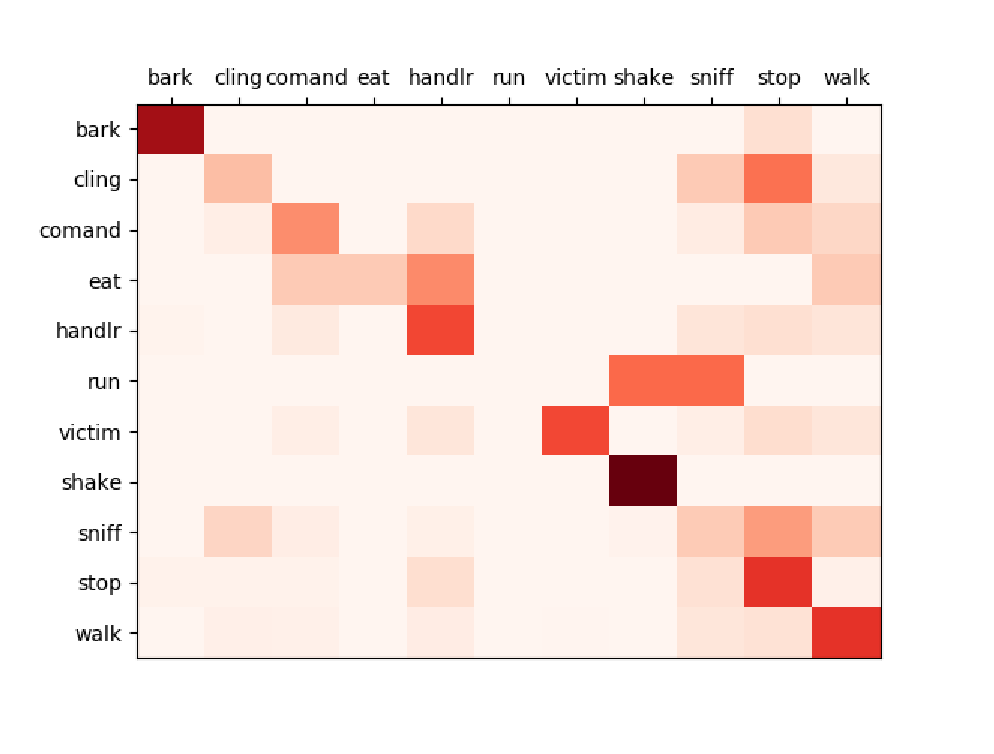
\includegraphics[scale=0.7]{./Figures/resque_optmean_result.eps}
    \caption{VGG16 pretrained modelとレスキュー犬訓練データセットoptical flow動画フレーム平均画像によるクラス分類のfinetuning結果}
    \label{sub_optresque_res}
  \end{center}
\end{figure}
